\chapter{Voxelwise Temporal Clustering Model}
\label{chapter:voxelwise}

\section{Introduction}

% motivate the idea of avoiding a priori region specification
The main limitation of data-driven models such as the Event-Based Model (section \ref{sec:ebm}), the Differential Equation Model (section \ref{sec:dem}) or the Disease Progression Score (DPS) (section \ref{sec:dps}) is that they use a small set of biomarkers that are obtained by averaging MRI or PET measures across all voxels or vertices in a Region of Interest (ROI). This can be problematic, especially if different parts of the ROI, say the hippocampus, are affected at different speeds or timepoints in the disease process. Therefore, moving to a voxel-wise approach would allow one to estimate the fine-grained spatial distribution of atrophy, which would give new insights into the disease process and enable more precise staging. A voxel-wise disease progression model by Bilgel et al. \cite{bilgel2016multivariate} (see section \ref{sec:bilgel_voxelwise}) has been recently proposed to mitigate this problem, that uses amyloid measures in each voxel as its input data.

% highlight the limitations of bilgel et al. and explain the quantum leap
The voxel-wise model by \cite{bilgel2016multivariate} has two limitations: (1) it does not show which areas of the brain have a similar progression dynamics; (2) the biomarker trajectories are assumed to be linear, which are not suitable given that many biomarkers such as amyloid or tau plateau after a certain point. Moreover, the model uses a spatial correlation function for modelling correlation between voxels. While this is necessary, due to the nature of the imaging data, it has been shown that in different types of dementia atrophy patterns match functional networks, which are not spatially connected \cite{seeley2009neurodegenerative}. 

In this work, we present a new disease progression model with single vertex resolution that avoids assumptions on spatial correlation. We combine unsupervised learning and disease progression modelling to identify clusters of vertices on the cortical surface, with no spatial constraints, that show a similar trajectory of atrophy over a particular patient cohort. This formulation enables us to gain new insights into the spatial structure of atrophy in different diseases and also provides a novel parcellation of the brain based on temporal change. Moreover, each cluster of vertices has a corresponding sigmoidal trajectory, which avoids the limitation of linear trajectories in \cite{bilgel2016multivariate}. 

We first show using simulated data that our model is able to recover the underlying clusters, trajectory parameters and subject stages. We then apply our model to cortical thickness vertex-wise measures using ADNI and DRC datasets and highlight the new insights the model can give. Finally, we validate our model using cross-validation and by correlating the subject stages with cognitive measures.

% We first show that our algorithm gives similar answers on the two independent typical AD datasets (ADNI and local dataset). Secondly, when modelling distincts disease populations (PCA vs AD), our method finds different atrophy patterns which broadly reflect the known spatial distribution of atrophy in each condition. Finally, using cross calidation on the ADNI data we show that the model is robustly recovering the same clusters and that the stages are clinically meaningful, as they correlate with four different cognitive tests.

\section{Methods}
\label{sec:vwdpm_methods}

\subsection{Model}
\label{sec:vwdpm_model}

% progresison score, affine transformation
We seek to identify groups of image vertices that show a common trajectory during the disease course, while simultaneously placing each visit from each subject within that disease course. In a similar way to \cite{jedynak2012,donohue2014estimating,schiratti2015mixed}, we estimate a time shift and speed (or rate) of progression for each subject. We relate these time shifts and progression speeds by assigning each subject a disease stage which we will refer to as the Disease Progression Score (DPS). In contrast to \cite{jedynak2012,donohue2014estimating,schiratti2015mixed}, which model temporal trajectories for a small set of biomarker measures based on \emph{a priori} defined ROIs, we model temporal trajectories for each vertex on the cortical surface. Each trajectory is a function of the disease progression score (i.e. disease stage) of a subject. We estimate each subjects' time shift, progression speed and each trajectory from the data. The disease progression score $s_{ij}$ for subject $i$ at visit $j$ is defined as a linear transformation of age $t_{ij}$:

\begin{equation}
\label{eq:dps_vwdpm}
 s_{ij} = \alpha_i t_{ij} + \beta_i
\end{equation}
% sigmoidal functions
where $\alpha_i$ and $\beta_i$ represent the speed of progression and time shift (i.e. disease onset) of subject $i$. 

Our model assumes that the cortical thickness at each vertex on the cortical surface follows a sigmoidal trajectory $f(s)$ given the disease progression score $s$. We also assume that vertices are grouped into $K$ clusters and we model a unique trajectory for each cluster $k \in [1, \dots, K]$, which will be referred to as cluster trajectories. The sigmoidal function for cluster $k$ is parametrised as $\theta_k = [a_k,b_k,c_k,d_k]$ where 

\begin{equation}
\label{eq:dps_vwdpm2}
 f(s;\theta_k) = \frac{a_k}{1+exp(-b_k(s-c_k))} + d_k
\end{equation}

For a given subject $i$ at visit $j$, the value $V_l^{ij}$ of its cortical thickness at vertex $l$ is a random variable that has an associated discrete latent variable $Z_l \in [1, \dots, K]$ denoting the cluster it was generated from. The value of $V_l^{ij}$ given that it was generated from cluster $Z_l$ can be modelled as:

% TODO cannot use Z_l for the index of theta and for a random variable, use smth like Z_l = z_l, but watch out later on not to have conflicts.

% model for one voxel and label
\begin{equation}
\label{eq:dps_vwdpm3}
 p(V_l^{ij} | \alpha_i, \beta_i, \theta_{Z_l}, \sigma_{Z_l}, Z_l) = N(V_l^{ij} | f(\alpha_i t_{ij} + \beta_i | \theta_{Z_l}), \sigma_{Z_l})
\end{equation}
where $N(V_l^{ij} | f(\alpha_i t_{ij} + \beta_i | \theta_{Z_l}), \sigma_{Z_l})$ represents the pdf of the normal distribution that models the measurement noise along the sigmoidal trajectory of cluster $Z_l$, having variance $\sigma_{Z_l}$. Next, we assume the measurements from different subjects are independent, while the measurements from the same subject $i$ at different visits $j$ are linked using the disease progression score from equation \ref{eq:dps_vwdpm}, because we estimate only two parameters ($\alpha_i$ and $\beta_i$) using the data from all visits $j$. Moreover, we also assume a uniform prior on $Z_l$. This gives the following model:

% all subj are independent
\begin{equation}
\label{eq:dps_vwdpm4}
 p(V_l, Z_l | \alpha, \beta, \theta, \sigma) = \prod_{(i,j) \in I} N(V_l^{ij} | f(\alpha_i t_{ij} + \beta_i | \theta_{Z_l}), \sigma_{Z_l})
\end{equation}
where $I = {(i,j)}$ represents the set of all the subjects $i$ and their corresponding visits $j$. Furthermore, $V_l = [V_l^{ij} | (i,j) \in I]$ is the 1D array of all the values for vertex $l$ across every subject and corresponding visit. Vectors $\alpha = [\alpha_1, \dots, \alpha_S]$ and $\beta = [\beta_1, \dots, \beta_S]$, where $S$ is the number of subjects, denote the stacked parameters for the subject shifts. Vectors $\theta = [\theta_1, \dots, \theta_K]$ and $\sigma = [\sigma_1, \dots, \sigma_K]$, with $K$ being the number of clusters, represent the stacked parameters for the sigmoidal trajectories and measurement noise specific to each cluster.

We further assume all vertex measurements to be spatially independent, giving the complete data likelihood:

% all vertices are independent
\begin{equation}
\label{eq:dps_vwdpm5}
 p(V, Z | \alpha, \beta, \theta, \sigma) = \prod_l^L \prod_{(i,j) \in I} N(V_l^{ij} | f(\alpha_i t_{ij} + \beta_i | \theta_{Z_l}), \sigma_{Z_l})
\end{equation}
where $V = [V_1, \dots, V_L]$, $Z = [Z_1, \dots, Z_L]$, $L$ being the total number of vertices on the cortical surface. We recall that we don't want to enforce spatial correlation between vertices as we are interested to see if vertices from distinct areas of the brain are grouped together in the same cluster. Our assumption is also justified by the fact that we smoothed the cortical thickness images in the preprocessing steps. We get the final model log likelihood for incomplete data by marginalising over the latent variables $Z$:
\begin{equation}
\label{eq:dps_vwdpm6}
 p(V|\alpha, \beta, \theta, \sigma) = \prod_{l=1}^L \sum_{k=1}^K p(Z_l = k) \prod_{(i,j) \in I} N(V_l^{ij} | f(\alpha_i t_{ij} + \beta_i | \theta_k), \sigma_k)
\end{equation}
Therefore, the parameters that need to be estimated are $\Theta = [\alpha, \beta, \theta, \sigma]$ where $\alpha$ and $\beta$ are the subject specific shifting parameters while $\theta$ and $\sigma$ are the cluster specific trajectory and noise parameters. 

\subsection{Fitting the Model using EM}
\label{sec:vwdpm_fitting_model}

Due to the summing over the latent variables $Z$, it is not possible to find a closed form solution to the maximum likelihood. Therefore, we fit our model using Expectation-Maximisation, which is suitable given the large number of data points and parameters that need to be estimated. 

% We therefore seek to maximize:
% \begin{equation}
% \label{eq:EMgen}
% \argmax_{\Theta} E_{Z|V,\Theta^{old}} [log\ p(V,Z|\Theta)] + log\ p(\Theta) 
% \end{equation}
% where $\Theta^{old} = (\alpha^{old}, \beta^{old}, \theta^{old}, \sigma^{old})$ and $log\ p(\Theta)$ is a prior on the parameters.

\subsubsection{E-step}

In the Expectation step we seek to estimate which cluster has generated each of the $L$ vertices, given the current estimates of the cluster parameters $\theta_k^{old}, \sigma_k^{old}$ as well as the subject specific shift parameters $\alpha_i^{old}, \beta_i^{old}$. More formally, we seek to find $p(Z|V,\Theta^{old}) = \prod_l^L p(Z_l|V_l,\Theta^{old})$, given our independence assumption between vertices. Let us denote by $z_{lk} = p(Z_l = k | V_l,\Theta^{old})$. We then have:

\begin{equation}
 z_{lk} =  \frac{\prod_{(i,j) \in I} N(V_l^{ij} | f(\alpha_i^{old} t_{ij} + \beta_i^{old} | \theta_k^{old}), \sigma_k^{old})}{\sum_{m=1}^K \prod_{i,j \in I} N(V_l^{ij} | f(\alpha_i^{old} t_{ij} + \beta_i^{old} | \theta_m^{old}), \sigma_m^{old})}
\end{equation}
Ignoring the normalisation factor, we take the log and expand the pdfs of the normal distributions. This results in the following update equation for the E-step:

\begin{equation}
 log\ z_{lk} \propto  -\frac{1}{2} log\ (2 \pi \left(\sigma_k^{old}\right)^2) |I| - \frac{1}{2\left(\sigma_k^{old}\right)^2} \sum_{(i,j) \in I} (V_l^{ij} - f(\alpha_i^{old} t_{ij} + \beta_i^{old} | \theta_k^{old}))^2 
\end{equation}
The original probabilities can be easily recovered by exponentiating them and then normalising with respect to their sum.

\subsubsection{M-step}

In the Maximisation step we try to find $\Theta = (\alpha, \beta, \theta, \sigma)$ that maximise $E_{Z|V,\Theta^{old}} [log\ p(V,Z|\Theta)]$. Since there is no closed-form solution, we perform successive refinements of $\theta_k$ for each cluster $k$ and $\alpha_i, \beta_i$ for each subject $i$ until convergence. 

In order to get the update rule for the trajectory parameters $\theta_k$ corresponding to cluster $k$ we need to maximise the expected log likelihood with respect to $\theta_k$. We get the following simplified optimisation problem:

\begin{equation}
 \label{eq:theta}
 \theta_k = \argmin_{\theta_k} \left[\sum_{l=1}^L z_{lk} \sum_{(i,j) \in I} (V_l^{ij} - f(\alpha_i t_{ij} + \beta_i | \theta_k))^2 \right] - log\ p(\theta_k) 
\end{equation}
A similar equation is also obtained for $\sigma_k$. After estimating $\theta$ and $\sigma$ for every cluster, we use the new values to estimate the subject specific parameters $\alpha$ and $\beta$. Let $S$ be the number of subjects and $\alpha_i$, $\beta_i$ be the rate and shift for subject $i \in S$. We again maximise the expected log likelihood with respect to $\alpha_i$, $\beta_i$ independently, and after further simplifications we obtain the following problem:

\begin{equation}
\label{eq:alpha}
 \alpha_i, \beta_i = \argmin_{\alpha_i, \beta_i}  \left[ \sum_{l=1}^L \sum_{k=1}^K z_{lk} \frac{1}{2\sigma_k^2} \sum_{j \in I_i} (V_l^{ij} - f(\alpha_i t_{ij} + \beta_i | \theta_k))^2\right] - log\ p(\alpha_i, \beta_i)
\end{equation}

In summary, at every single M-step, we iterate between solving for $\theta$, $\sigma$ and solving for $\alpha$, $\beta$ using numerical optimisation until convergence. Due to the use of numerical optimisation, we are not guaranteed to find the global maxima for the expected log likelihood, but it has been shown that EM still works if we only find an increase in the log-likelihood \cite{bishop2006pattern}. This approach that involves a partial M-step is called Generalised EM.

\subsection{Initialisation and Implementation}
\label{sec:vwdpm_initialisation}
% initialisation
The optimisation algorithm is given in figure \ref{fig:algo_vwdpm}. Before starting the fitting process, we need to initialise $\alpha$, $\beta$ and the clustering probabilities $z_{lk}$. We set $\alpha_i$ and $\beta_i$ to be 1 and 0 respectively for each subject. We initialise $z_{lk}$ using k-means clustering using vectors $V_l$ having $|I|$ number of samples and $L$ features. Furthermore, as already explained in \cite{jedynak2012}, the scale of the DPS is arbitrary so we standardise the scores at each EM iteration such that the DPS of controls have a mean $\mu_N$ of zero and a standard deviation $\sigma_N$ of 1. This also requires a rescaling of the cluster parameters $\theta_k$.

In our implementation, we run the main EM loop until convergence of the clustering probabilities $z_{lk}$. At each M-step we also perform successive refinements of parameters $\theta$, $\alpha$ and $\beta$ using equations \ref{eq:theta}, \ref{eq:alpha} until convergence. For the numerical optimisation we used the Broyden-Fletcher-Goldfarb-Shanno (BFGS) algorithm that makes use of the first derivative of the objective function. In all datasets analysed, the method converges after maximum 25 EM iterations.\\

\begin{figure}
\begin{algorithm}[H]
%  \KwData{this text}
%  \KwResult{how to write algorithm with \LaTeX2e }
 Initialise $\alpha$, $\beta$, $z_{lk}$ \\
 \tcp*[l]{Outer loop}
%  $ a=1$\\ 
 \While{$z_{lk}$ not converged}{ 
  %M-step\\
   \tcp*[l]{M-step}
  \While{$\theta$, $\sigma$, $\alpha$, $\beta$ not converged}{
   \tcp*[l]{Optimise trajectories}
    \For{$k=1$ to $K$}{
      ${\theta_k = \argmin_{\theta_k} \sum_{l=1}^L z_{lk} \sum_{(i,j) \in I} (V_l^{ij} - f(\alpha_i t_{ij} + \beta_i | \theta_k))^2  - log\ p(\theta_k)}$\\
      ${\sigma_k^2 = \frac{1}{|I|} \sum_{l=1}^L z_{lk} \sum_{(i,j) \in I} (V_l^{ij} - f(\alpha_i t_{ij} + \beta_i | \theta_k))^2 - log\ p(\sigma_k)}$
    }
     \tcp*[l]{Optimise subject shifts}
    \For{$i=1$ to $S$}{
      ${\alpha_i, \beta_i = \argmin_{\alpha_i, \beta_i}  \left[ \sum_{l=1}^L \sum_{k=1}^K z_{lk} \frac{1}{2\sigma_k^2} \sum_{j \in I_i} (V_l^{ij} - f(\alpha_i t_{ij} + \beta_i | \theta_k))^2\right] - log\ p(\alpha_i, \beta_i)}$
    }
     \tcp*[l]{Re-scale subject shifts}
    \For{$i=1$ to $S$}{
      $\alpha_i = \frac{\alpha_i}{\sigma_N}, \beta_i = \frac{\beta_i - \mu_N}{\sigma_N}$
    }
     \tcp*[l]{Make trajectory parameters identifiable}
    \For{$k=1$ to $K$}{
      $\theta_k = \mbox{make\_identifiable}(\theta_k)$\\
      $\theta_k = \mbox{rescale}(\theta_k)$
    }
  }
  %E-step\\
   \tcp*[l]{E-step}
  \For{$l = 1$ to $L$}{
    \For{$k = 1$ to $K$}{
      ${ z_{lk} \propto  -\frac{1}{2} log\ (2 \pi \sigma_k^2) |I| - \frac{1}{2\sigma_k^2} \sum_{(i,j) \in I} (V_l^{ij} - f(\alpha_i t_{ij} + \beta_i | \theta_k))^2  }$
    }
  }
 }
\end{algorithm}
\caption{The model fitting algorithm.}
\label{fig:algo_vwdpm}
\end{figure}

\section{Simulation results}
\label{sec:vwdpm_simulations}

% method
We first tested the model in a toy scenario using synthetic data to see how well the cluster probabilities, trajectories and subject shifts are recovered. We generated our data as follows:
\begin{enumerate}
 \item sampled age and shift parameters from 300 subjects with 4 timepoints (each timepoint 1 year apart), with $t_{i1} \sim U(40,80)$, $\alpha_i \sim N(1, 0.05)$, $\beta_i \sim N(0, 10)$
 \item generated three sigmoids with different center points and slopes (Fig. \ref{fig:synThetaRes}, red lines). 
 \item generated a random cluster assignment for $L = 1,000$ vertices, i.e. every vertex $l$ was assigned to a cluster $a[l] \in \{1,2,3\}$
 \item sampled a set of $L$ perturbed trajectories $\theta_l$ from each of the original trajectories, one for each vertex (Fig. \ref{fig:synThetaRes}, gray lines)
 \item sampled subject data for every vertex $l$ from its corresponding perturbed trajectory $\theta_l$ with $\sigma_l = 0.5$
\end{enumerate}
To fit the data we used a uniform prior on the parameters $\theta$ and $\sigma$ and an informative prior on $\alpha$ and $\beta$, with $p(\alpha_i) \sim \Gamma(49,70)$ and $\beta_i \sim N(0,1)$. We also normalised age to have a mean of 0 and standard deviation of 1 and rescaled the DPS and cluster trajectories accordingly. After convergence, we calculated the agreement between the final clustering probabilities and the true clustering assignments as $A = \frac{1}{L}\sum_{l=1}^L p(Z_l = a[l])$. However, the recovered clusters can be found in a permuted order, so we used the permutation that yielded the highest agreement $A$. The method also requires us to set the number of clusters \emph{a priori}, so in order to find the optimal number of clusters we used model selection with the Bayesian Information Criterion (BIC). 

% Results
The BIC analysis correctly predicted 3 clusters for this synthetic experiment. Using three clusters, we also obtained a clustering agreement of $A = 1.0$. Figure \ref{fig:synThetaRes} shows the original trajectories and the recovered trajectories using our model, plotted against the disease progression score on the x-axis and the vertex value on the y-axis. Moreover, in Fig. \ref{fig:synShiftRes} we plotted the recovered DPS of each subject along with the true DPS. 

% Conclusion
The results show that the model accurately estimated which clusters generated each vertex. Moreover, the recovered trajectories are close to the true trajectories, with some errors for the trajectories corresponding to clusters 1 and 2. The recovered DPS also shows good agreement with the true DPS, with the exception of a few subjects with DPS greater than 2.5. This is explained by the fact that there is not enough signal in that DPS range in terms of trajectory dynamics (i.e. trajectories are mostly flat). The simulation confirms that our model is able to recover the hidden clusters, trajectory parameters and the subject specific parameters. However, more realistic simulations with varying noise levels and numbers of clusters are required to understand the limitations of the model and find out when it fails to recover the true parameters. 


\begin{figure}
\begin{subfigure}[b]{0.75\textwidth}
  \hspace{-2em}
  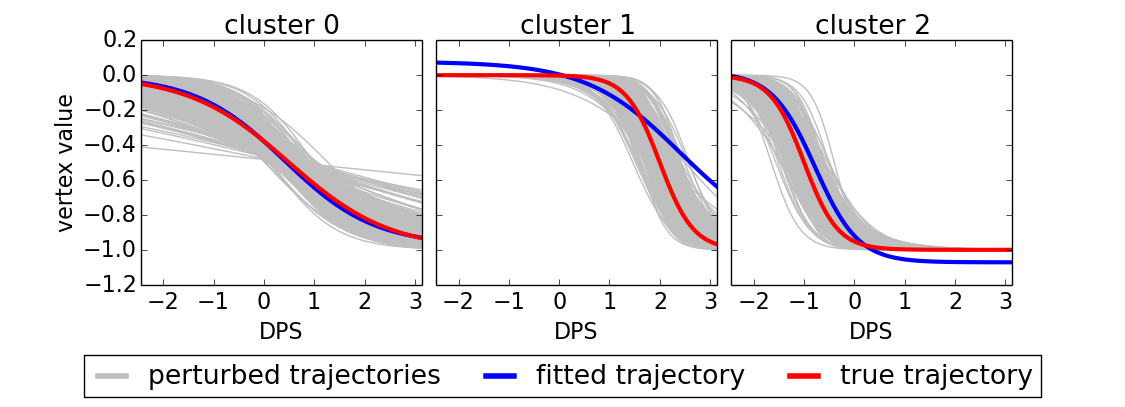
\includegraphics[width=1.15\textwidth]{images/vwdpm//synThetaRes_gensigInitk-meansCl3Pr1Ra0_VWDPMStd.png}
  \caption{}
  \label{fig:synThetaRes}
\end{subfigure}
\hspace{-1em}
\begin{subfigure}[b]{0.24\textwidth}
\centering
  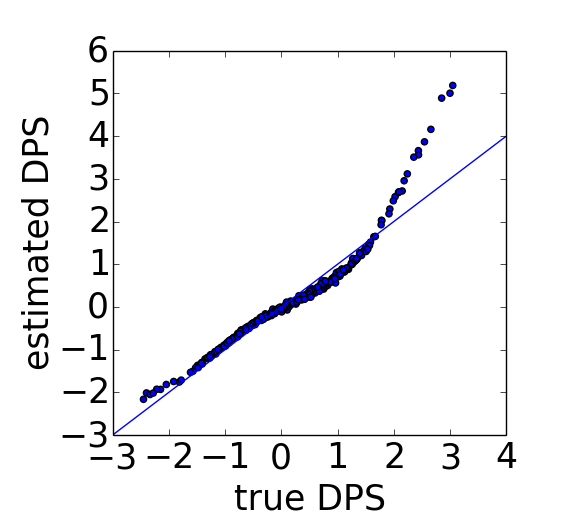
\includegraphics[width=1.2\textwidth]{images/vwdpm/synShiftsRes_gensigInitk-meansCl3Pr1Ra0_VWDPMStd.png}
    \vspace{0.7em}
  \caption{}
  \label{fig:synShiftRes}
\end{subfigure}
\caption{(a) Reconstructed temporal trajectories (blue) from the synthetic data along with the true trajectories (red). The data was generated from the perturbed trajectories, which in turn were generated from the true trajectories. (b) Estimated subject-specific disease progression scores compared to the true scores.}
\end{figure}

\section{Experimental results}
\label{sec:vwdpm_results}

\subsection{Data acquisition and preprocessing}

We analysed cortical thickness measures from two datasets: ADNI and DRC dataset. For ADNI, we downloaded from http://adni.loni.usc.edu/ all T1 MRI images that have undergone gradwarping, intensity correction and scaling for gradient drift. We included subjects that had at least 4 scans, in order to ensure we get a robust estimate of the subject specific parameters. This resulted in 328 subjects with an average number of 4.95 scans each. The DRC dataset consisted of T1 MRI scans from 31 healthy controls, 32 PCA and 23 typical typical AD subjects with at least 3 scans each and an average of 5.26 scans per subject.

% freesurfer pipeline
On both datasets, in order to extract reliable thickness measures we ran the Freesurfer longitudinal pipeline \cite{reuter2012within}, which first registers the MRI images to an unbiased within-subject template space using inverse-consistent registration. The longitudinally registered images were then registered to the Freesurfer template and smoothed at various full-width/half-max (FWHM) values. We used the FWHM zero level and for each vertex we averaged the thickness levels from both hemispheres. Finally, we standardised the data from each vertex with respect to the values of that vertex in the control population.  Each of the final images had a resolution of 163,842 vertices on the cortical surface. 


\subsection{Results with ADNI and DRC datasets}
\label{sec:vwdpm_results_sub}

% Motivation: 
% 1. see how the patterns of atrophy look in the two diseases tAD and PCA look like. 
% 2. see if similar results are obtained on two independent datasets
% 3. see if different atrophy patterns are obtained in tAD vs PCA, and if they match previous studies.
Using ADNI and DRC datasets, we were interested to find out the spatial distribution of cortical atrophy, as well as the rate and timing of this atrophy process. In particular, we would like to find out: (1) if we get similar results using our model on two independent tAD datasets: ADNI and DRC datasets and (2) if we get different patterns of atrophy on distinct diseases (tAD and PCA) that match previous studies. 

% Results
BIC analysis predicted that the optimal number of clusters is two for the ADNI cohort and three for both tAD and PCA subjects from the DRC cohort. In order to make the results easily comparable across the different datasets, we ran all experiments using 3 clusters. Fig. \ref{fig:adniClust} shows the results of our model using all ADNI subjects, where we coloured points on the cortical surface according to the cluster they most likely belong to. We assigned a colour to each cluster according to the slope of its corresponding trajectory, ranging from red (high slope suggesting a fast rate of atrophy) to blue (low slope suggesting a slow rate of atrophy). In Fig. \ref{fig:adniTraj} we also show the resulting cluster trajectories with samples from the posterior distribution of each $\theta_k$. We repeated the same analysis on the DRC cohort, separately for the tAD subjects (Fig. \ref{fig:drcClustAD} and \ref{fig:drcTrajAD}) and PCA subjects (Fig. \ref{fig:drcClustPCA} and \ref{fig:drcTrajPCA}). 

% Conclusions - first talk about tAD then about PCA
We notice that in tAD subjects using both ADNI and the DRC dataset (Fig. \ref{fig:clustTrajAll}), there is widespread atrophy in most temporal, parietal and frontal areas (red cluster), with the notable exception of the motor cortex and the occipital lobe. These patterns of atrophy are similar across the two different datasets. Moreover, the spatial distribution of cortical thinning found with our technique resembles results from previous longitudinal studies \cite{dickerson2009cortical,thompson2001cortical}. However, in contrast to those approaches, our model gives insight into the timing, rate and extent of atrophy.

In the PCA subjects (Fig. \ref{fig:drcClustPCA}), we find that the atrophy is more focused on the posterior part of the brain, mostly the posterior parietal and occipital, with more limited spread in the superior temporal and inferior frontal. This is in contrast with the tAD patterns in the other datasets, that lacks the focus on posterior parietal and occipital regions. This posterior pattern of atrophy also matches previous findings in the literature \cite{crutch2012posterior}. For all datasets, we find that the cluster trajectories differ less in timing and more in the slope and minima/maxima values at which they plateau (Fig. \ref{fig:adniTraj}, \ref{fig:drcTrajAD}, \ref{fig:drcTrajPCA}). Our model therefore predicts that regions on the cortical surface are all affected roughly at the same time, but the rate and extent to which they are affected is different.   

\newcommand{\scalingFactor}{1}

\newcommand{\gradLimLeft}{-1.6}
\newcommand{\gradLimRight}{1.6}

% \newcommand{\scalingFactorLeftFig}{1.2}
\newcommand{\scalingFactorBrains}{1}
\newcommand{\scalingFactorTraj}{1.1}

% FWHM0 avg thickness map MCI & AD
\begin{figure}[h]
  \centering

  % do the legend colorbar
  \begin{subfigure}[b]{\textwidth}
   \centering
  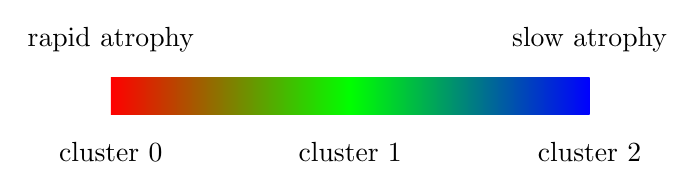
\begin{tikzpicture}[scale=1.9]
    \shade[left color=red,right color=green] (\gradLimLeft,2.5) rectangle (0,2.75);
    \shade[left color=green,right color=blue] (0,2.5) rectangle (\gradLimRight,2.75);
    \node[inner sep=0] (corr_text) at (\gradLimLeft,2.25) {cluster 0};
    \node[inner sep=0] (corr_text) at (0,2.25) {cluster 1};
    \node[inner sep=0] (corr_text) at (\gradLimRight,2.25) {cluster 2};
    \node[inner sep=0] (corr_text) at (\gradLimLeft,3) {rapid atrophy};
    \node[inner sep=0] (corr_text) at (\gradLimRight,3) {slow atrophy};
  \end{tikzpicture}
%     \caption{}
%       \label{fig:adniClust}
  \vspace{1em}
  \end{subfigure}
  
  %%%%%%%%%%%%%%%%%%% BRAINS %%%%%%%%%%%%%%5%%%%%%
  
  \begin{subfigure}[b]{0.3\textwidth}
   \centering
  \begin{tikzpicture}[scale=\scalingFactor, every node/.style={scale=\scalingFactor}]
    \node[inner sep=0] (image) at (0,0) {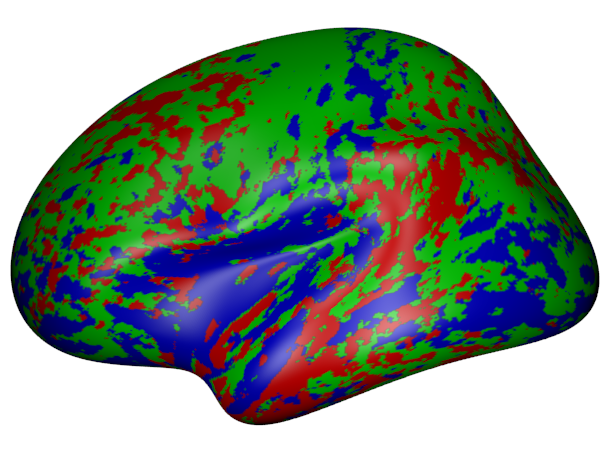
\includegraphics[width=\scalingFactorBrains\textwidth]{images/vwdpm/blend14_adniThavgFWHM0InithistCl3Pr0Ra1_VWDPMStd.png}}; 
    \node[inner sep=0] (label) at (0,3.5) {tAD - ADNI};
  \end{tikzpicture}
    \caption{}
      \label{fig:adniClust}
  \end{subfigure}
   \begin{subfigure}[b]{0.3\textwidth}
  \centering
  \begin{tikzpicture}[scale=\scalingFactor]
    \node[inner sep=0] (corr_text) at (0,0) {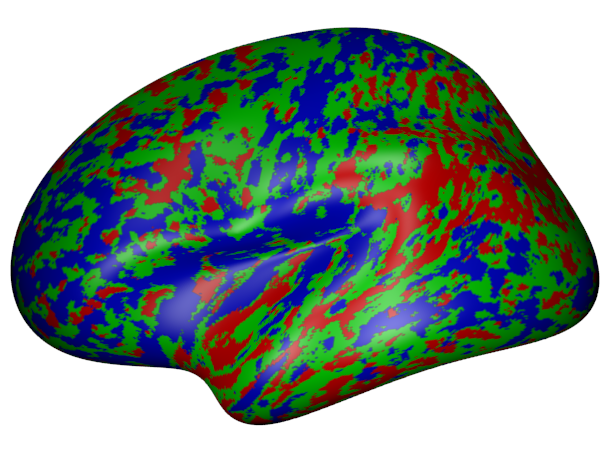
\includegraphics[width=\scalingFactorBrains\textwidth]{images/vwdpm/drcThavgFWHM0InithistCl3Pr0Ra1_VWDPMStdAD_blend24.png}};
    \node[inner sep=0] (label) at (0,3.5) {tAD - DRC dataset};
  \end{tikzpicture}
    \caption{}
      \label{fig:drcClustAD}
  \end{subfigure}
   \begin{subfigure}[b]{0.3\textwidth}
  \centering
  \begin{tikzpicture}[scale=\scalingFactor, every node/.style={scale=\scalingFactor}]
    \node[inner sep=0] (corr_text) at (0,0) {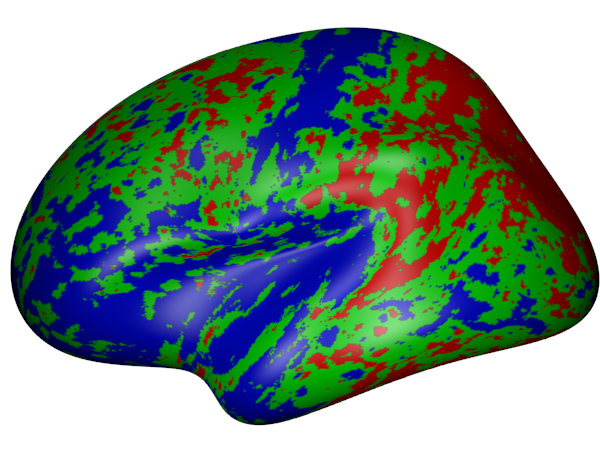
\includegraphics[width=\scalingFactorBrains\textwidth]{images/vwdpm/drcThavgFWHM0InithistCl3Pr0Ra1_VWDPMStdPCA_blend24.png}};
    \node[inner sep=0] (label) at (0,3.5) {PCA - DRC dataset};
  \end{tikzpicture}
    \caption{}
      \label{fig:drcClustPCA}
  \end{subfigure}
  
  %%%%%%%%%%%%%%%%%%%%%% trajectories %%%%%%%%%%%%%%%%%%%%%%%
  
    \begin{subfigure}[b]{0.3\textwidth}
    \centering
%     \vspace{-2em}
    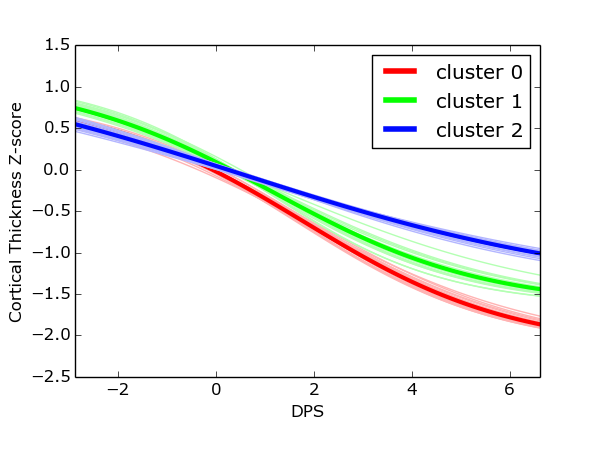
\includegraphics[width=\scalingFactorTraj\textwidth]{images/vwdpm/trajSamplesOneFig_adniThavgFWHM0InithistCl3Pr0Ra1_VWDPMStd.png}
    \caption{}
      \label{fig:adniTraj}
  \end{subfigure}
      \begin{subfigure}[b]{0.3\textwidth}
    \centering
%     \vspace{-2em}
    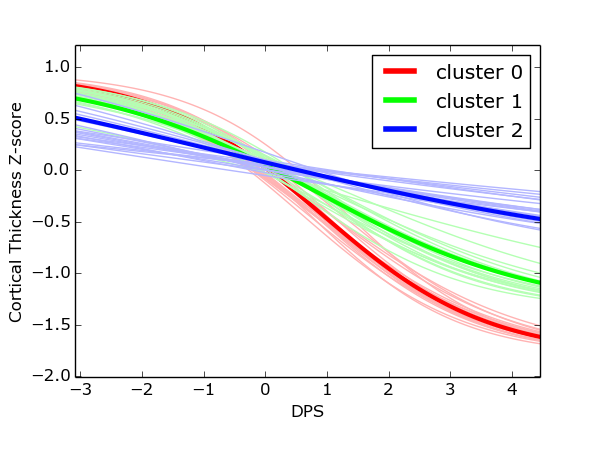
\includegraphics[width=\scalingFactorTraj\textwidth]{images/vwdpm/trajSamplesOneFig_drcThavgFWHM0InithistCl3Pr0Ra1_VWDPMStdAD.png}
    \caption{}
      \label{fig:drcTrajAD}
  \end{subfigure}
    \begin{subfigure}[b]{0.3\textwidth}
    \centering
%     \vspace{-2em}
    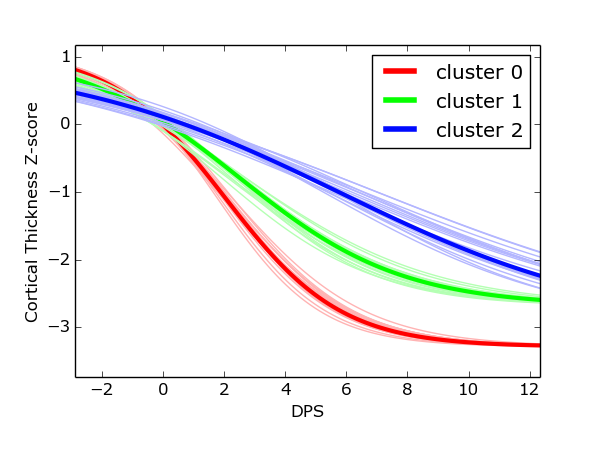
\includegraphics[width=\scalingFactorTraj\textwidth]{images/vwdpm/trajSamplesOneFig_drcThavgFWHM0InithistCl3Pr0Ra1_VWDPMStdPCA.png}
    \caption{}
      \label{fig:drcTrajPCA}
  \end{subfigure}
  
  \caption{(a) Clustering results on the ADNI data using our model, where each cluster is coloured according to the slope of its corresponding trajectory, from red (high slope suggesting very affected areas) to blue (low slope suggesting less affected areas). (d) The corresponding trajectories and samples from the posterior distribution of the trajectory  parameters for the three clusters in ADNI. The same analysis is shown also for (b, e) tAD subjects from the DRC cohort and (c, f) PCA subjects from the DRC cohort.}
  \label{fig:clustTrajAll}

\end{figure}

\subsection{Model Validation}
\label{sec:vwdpm_validation}

% motivation, i.e. what we wanted to test
We tested robustness of the model by performing 10-fold cross validation (CV) on ADNI. Our motivation was to test the following: (1) if similar spatial clustering is estimated at each fold, as quantified by Dice score overlap (2) if the stages of the test subjects were consistent (i.e. were increasing for follow-up visits) and (3) if the stages of test subjects are clinically meaningful, by correlating them with cognitive tests such as Clinical Dementia Rating Scale - Sum of Boxes (CDRSOB), Alzheimer's Disease Assessment Scale - Cognitive (ADAS-COG), Mini-Mental State Examination (MMSE) and Rey Auditory and Verbal Learning Test (RAVLT).

% results 
Fig \ref{fig:ADNICVbrains} shows the clusters that were estimated at each fold from the training data only. Moreover, in Fig. \ref{fig:stagingConsist} we plot the estimated DPS (i.e. disease stage) of each subject from the test set against their age.

% conclusion
The results in Fig. \ref{fig:ADNICVbrains} prove that the model is robust in cross-validation, as the estimated clusters are all very similar across folds. The average Dice scores we obtained across all pairs of folds were 0.89, 0.89 and 0.90 for clusters 0, 1 and 2 respectively. Furthermore, 84\% of the subjects analysed show increased stages across their follow-up visits, proving that the estimated stages are mostly consistent. Finally, the stages of test subject correlate with clinical measures such as CDRSOB ($\rho = 0.41$, $p < 1e-66$), ADAS-COG ($\rho = 0.40$, $p < 1e-62$), MMSE ($\rho = 0.39$, $p < 1e-58$) and RAVLT ($\rho = 0.35$, $p < 1e-46$), demonstrating that the stages have clinical validity.

\newcommand{\outFoldADNICVbrains}{images/vwdpm/crossvalid/adniThavgFWHM0Initk-meansCl3Pr0Ra1_VWDPMMean}

\begin{figure}[h]
    \centering
    
    \begin{subfigure}[b]{0.19\textwidth}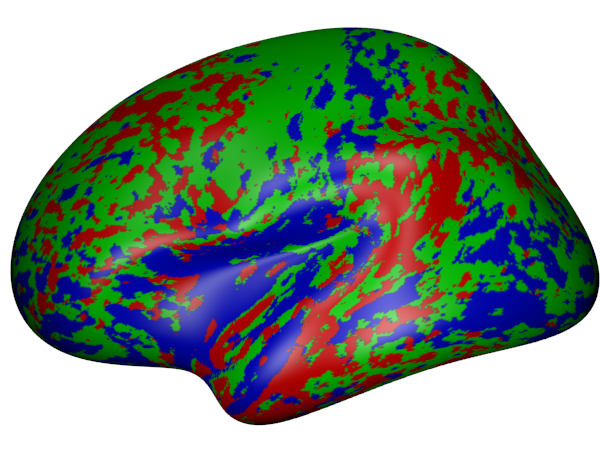
\includegraphics[width=\textwidth]{\outFoldADNICVbrains/blend0.png}\end{subfigure}
    \begin{subfigure}[b]{0.19\textwidth}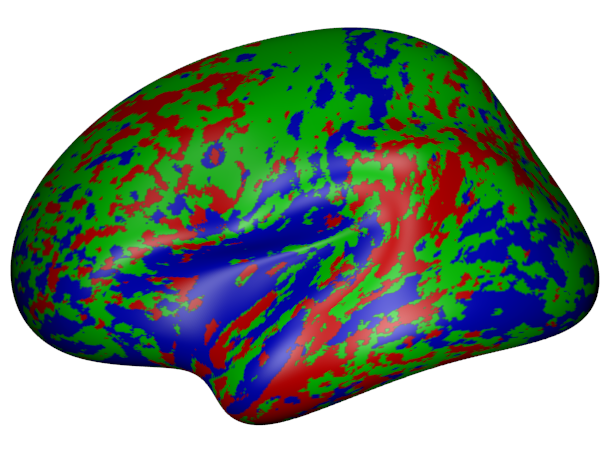
\includegraphics[width=\textwidth]{\outFoldADNICVbrains/blend1.png}\end{subfigure}
    \begin{subfigure}[b]{0.19\textwidth}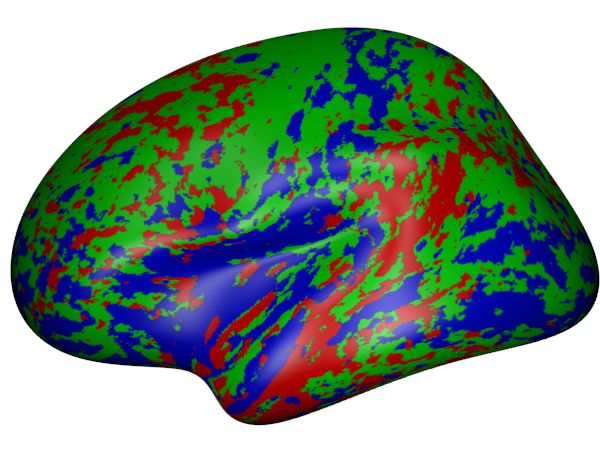
\includegraphics[width=\textwidth]{\outFoldADNICVbrains/blend2.png}\end{subfigure}
    \begin{subfigure}[b]{0.19\textwidth}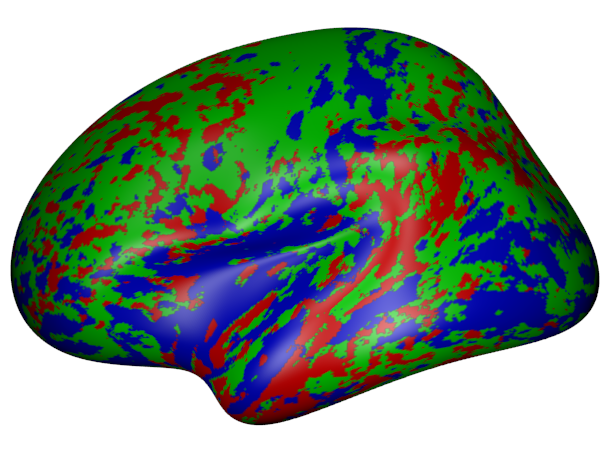
\includegraphics[width=\textwidth]{\outFoldADNICVbrains/blend3.png}\end{subfigure}
    \begin{subfigure}[b]{0.19\textwidth}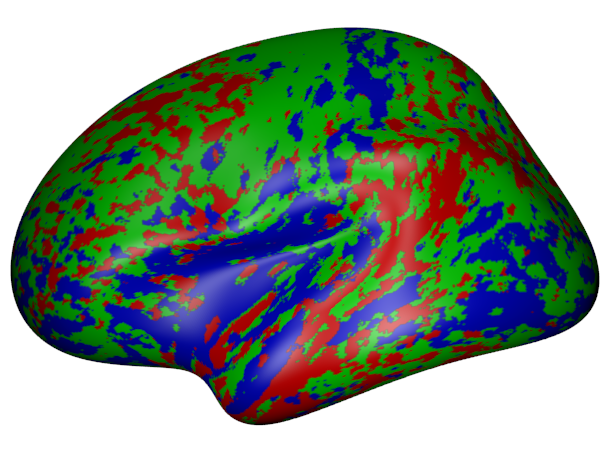
\includegraphics[width=\textwidth]{\outFoldADNICVbrains/blend4.png}\end{subfigure}
    \begin{subfigure}[b]{0.19\textwidth}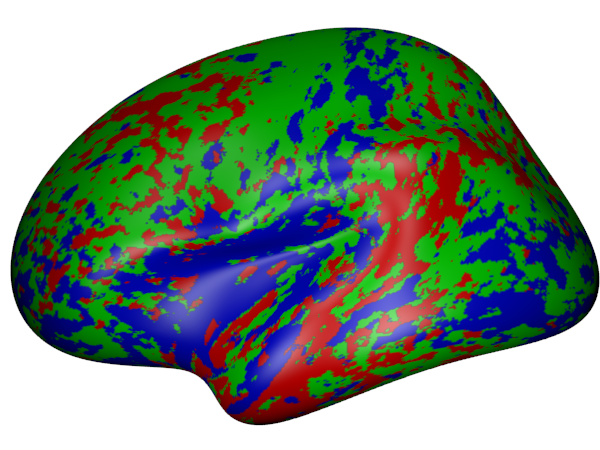
\includegraphics[width=\textwidth]{\outFoldADNICVbrains/blend5.png}\end{subfigure}
    \begin{subfigure}[b]{0.19\textwidth}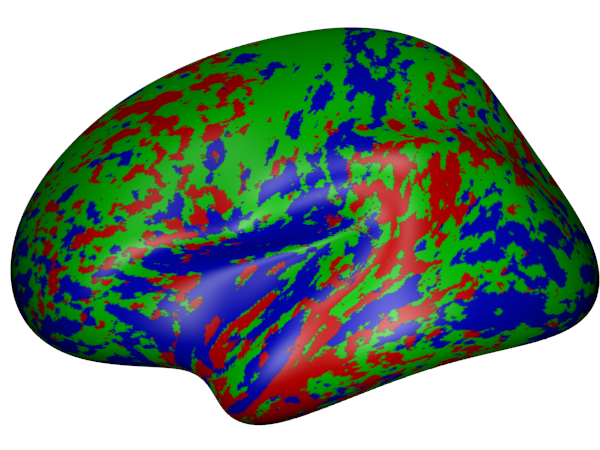
\includegraphics[width=\textwidth]{\outFoldADNICVbrains/blend6.png}\end{subfigure}
    \begin{subfigure}[b]{0.19\textwidth}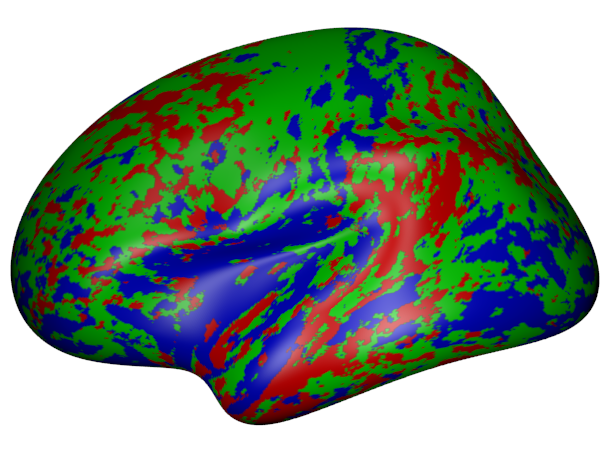
\includegraphics[width=\textwidth]{\outFoldADNICVbrains/blend7.png}\end{subfigure}
    \begin{subfigure}[b]{0.19\textwidth}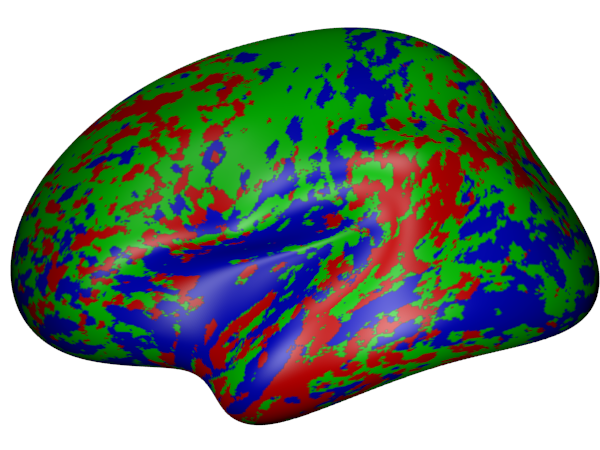
\includegraphics[width=\textwidth]{\outFoldADNICVbrains/blend8.png}\end{subfigure}
    \begin{subfigure}[b]{0.19\textwidth}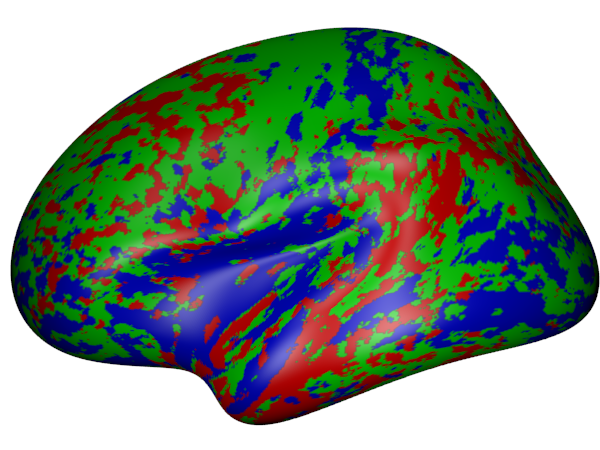
\includegraphics[width=\textwidth]{\outFoldADNICVbrains/blend9.png}\end{subfigure}
    
    \caption{Clusters estimated for each of the 10 cross-validation folds in ADNI. As before, each cluster is coloured according to the slope of its corresponding trajectory, from red (high rate of atrophy) to blue (low rate of atrophy).}
    \label{fig:ADNICVbrains}
\end{figure}


\begin{figure}[h]
    \centering
    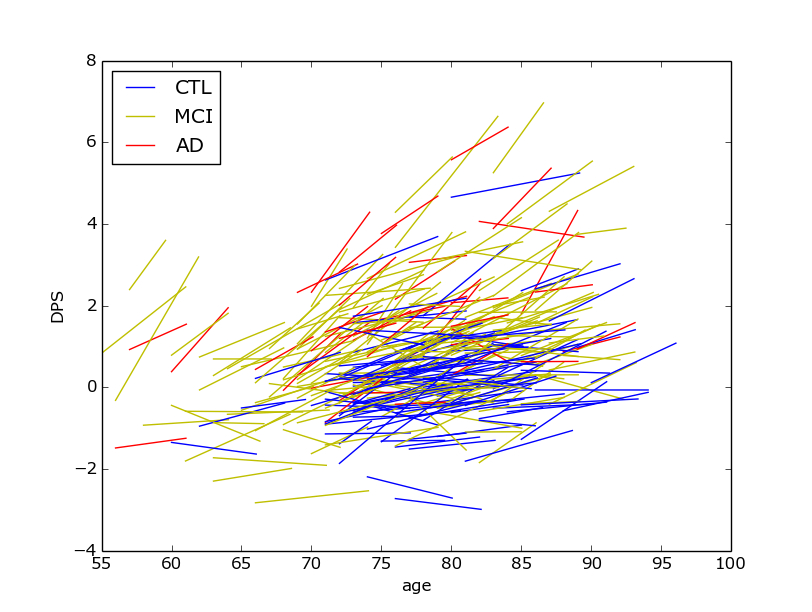
\includegraphics[width=0.5\textwidth]{images/vwdpm/crossvalid/stagingConsist_adniThavgFWHM0Initk-meansCl3Pr0Ra1_VWDPMMean.png}
    \caption{The disease progression score for each subject from the ADNI dataset estimated during 10-fold cross validation. Each line represents an individual $i$ with different visits $j$. Later visits generally have a higher corresponding stage.}
    \label{fig:stagingConsist}
\end{figure}

\section{Discussion}
\label{sec:vwdpm_discussion}

% summary -> other types of data -> not regress against age -> disease progression space -> model worked ok -> stages better than with static ROIs
We presented a model of disease progression that clusters vertex-wise measures of cortical thickness based on similar temporal dynamics. The model highlights, for the first time, groups of cortical vertices that exhibit a similar temporal trajectory over the population. This provides a new way to parcellate the brain that is specific to the temporal trajectory of a particular disease. The model also finds the optimal temporal shift and progression speed for every subject. We have applied it to cortical thickness vertex-wise data from ADNI and DRC cohorts. Our model found similar patterns of atrophy dynamics in the tAD subjects using two independent datasets. Moreover, it also found different patterns of atrophy dynamics on two distinct diseases: typical AD and PCA. 

% Limitations of the model
% a priori # of clust -> but can do BIC maximisation -> traj assumed sigmoidal -> but can use non-parametric curves -> Bias due to z-score normalisation - > susceptible to registration errors
The model has some limitations. First of all, we have assumed that cluster trajectories follow sigmoidal shapes, which might not be the case for many types of biomarkers such as cortical thickness. Another limitation of the model is that it assumes all subjects follow the same disease progression pattern, which might not be the case in heterogeneous datasets such as ADNI or the DRC cohort. Furthermore, the data we analysed has been standardised with respect to controls, which can introduce biases due to the fact that controls might already show some abnormalities in cortical thickness.

% future work on technical improvements, motivated by the limitations mentioned before
There are several potential avenues of future research. While we have only used the model for studying cortical thickness, one can also apply it to other types of data such as amyloid images or Jacobian compression maps. On the methodological side, the assumption of sigmoidal trajectories can be avoided using non-parametric curves such as Gaussian Processes or self-modelling regression techniques \cite{donohue2014estimating}. One could also model different progression dynamics for distinct groups in the population by clustering subjects together like the approach of \cite{young2015multiple}. The analysis could also be improved by using only amyloid negative controls for data standardisation.

% potential impact, clinical applications, work required to get there
Our approach can be used for accurately predicting and staging neurodegenerative disease progression. This is promising for patient prognosis, as well as in clinical-trials for assessing efficacy of a putative treatment for slowing down the degeneration process.